\documentclass{ctexart}
\usepackage[hmargin=1.1in,vmargin=1in]{geometry}
\usepackage{amsmath,amssymb}
\usepackage{multirow}
\usepackage{graphicx}
\usepackage[defaultmono]{droidsansmono}

\title{《信号处理导论》课程报告五}
\input{personal_info/info.tex}

\begin{document}
    \maketitle

    \section{我学到了哪个知识点?}

    傅里叶变换。傅里叶变换可以将一个关于时间的函数(时域上的信号)转换为一个关于频率(或角频率)的信号。基于被变换
    函数的不同,傅里叶变换共有四种情况,如下表所示:

    \begin{table}[h]
        \centering
        \caption{四种不同的傅里叶变换情况}
        \begin{tabular}{|*{2}{c|}}
            \hline
            原函数情况 & 变换情况 \\ \hline
            连续周期 & 离散非周期 \\
            连续非周期 & 连续非周期 \\
            离散周期 & 离散周期 \\
            离散非周期 & 连续周期 \\ \hline
        \end{tabular}
    \end{table}

    \section{我之前是怎么想的?}

    原先在学习算法竞赛时了解到有一种``快速傅里叶变换''算法,可以实现在 $O(n \log n)$ 时间内求两个 $n$ 次多项式
    的乘积。当时只了解到这个算法有三步,其中第一步是离散傅里叶变换:将一个 $n$ 次多项式转化为点值表达式;最后一步是
    离散傅里叶逆变换:将一个 $n$ 次多项式从其点值表达式转化回系数表达式。

    \section{我之前的想法怎么样?}

    以偏盖全。当时只了解到离散傅里叶变换,所以认为傅里叶变换只包括离散傅里叶变换和离散傅里叶逆变换,并且认为它的作用
    仅限于转换多项式的表达形式。实际上,将多项式在两种形式之间转换只是傅里叶变换的一个应用,离散傅里叶逆变换可以将
    一个离散序列从频域转换到时域,而离散傅里叶变换实际上是为了便于计算机处理,人为将一个有限离散序列(显然是非周期序
    列)延拓成了一个周期离散序列,从而使得它能够变换成频域上的离散周期序列(并且不需要进行积分等复杂操作)。

    \section{我应该怎样想才对?}

    傅里叶变换在信号处理中最大的作用在于,它能够将某个信号在时域与频域相互转换,这在很多场合很有用。比如说当我们需要
    研究某段音频,去除其中的杂音时,我们就可以先对采集到的音频信号做一次离散傅里叶变换(计算机只能采集到离散有限的音
    频信号),将杂音对应的那部分频率的信号删除,然后再对得到的新的频域信号做一次离散傅里叶逆变换,将其转换回时域信号
    使得计算机可以播放该信号(的一个周期)。

    另外,快速傅里叶变换算法中,第一步实质上就是将两个多项式时域信号转换为了频域上的信号(的一个周期),第二步利用傅
    里叶变换的频域卷积定理(或者按运算需要采用其他定理)对两个频域信号进行运算,然后第三步再将这个频域信号转换回到时
    域上,还原成系数表示的多项式。这也一定程度解释了为什么这个算法中第一步得到的``点值''的点一定是 $n$ 次单位根。

    \section{我应该怎样用上它?}

    各种傅里叶变换的推导过程实际上是对``信号正交分解''的一次又一次推广。这实际上再一次强调了``由已知求未知''的重要
    性;此外,傅里叶变换可以说是``沟通时域与频域的桥梁'',也教会我们看待事物要从多个角度去分析,才能更好地解决问题。

    \section*{字数统计}

    \begin{center}
        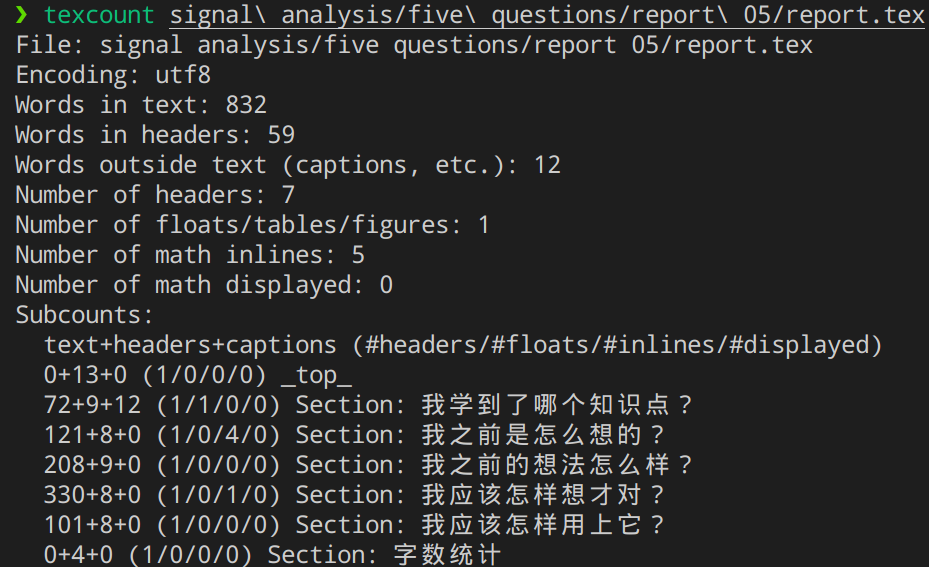
\includegraphics[width=0.8\textwidth]{pics/texcount.png}
    \end{center}
\end{document}